\documentclass{article}
\usepackage{graphicx} % Required for inserting images
\usepackage[margin=2.5cm]{geometry}
\usepackage{xcolor}
\usepackage{amsmath}
\usepackage{amssymb,amsthm}

\usepackage{enumitem}


\title{MesoCardio}
\author{Titouan Giraudon}
\date{September 2026}

\begin{document}

\maketitle
\newpage

\section{Muscle structure and mechanics}

\subsection{Quick description}
\begin{itemize}
    \item \textbf{Sarcomere} can be described as :\\
    Z disc — I band — A band — I band — Z disc
    \item \textbf{Sarcomere} is the basic unit of contraction, and when thousands of these units are linked together end-to-end, they form the long, continuous strand called a \textbf{myofibril}
    \item During muscle contraction, \textbf{actin} slides toward the center of the sarcomere (toward the M line by the myosin heads); the filaments themselves do not shorten, it is caused by the action of the molecular motor \textbf{myosin II}
    \item \textbf{A band} : Myosin and actin overlap, the length remains constant because the myosin filament doesn’t change length and it is located around the entire length of the myosin filament. It contains the H zone and the M line (dark band)
    \item \textbf{I band} : Actin only, length shortens, is located on either side of the Z disc (light band)
    \item \textbf{H zone} : it's the central region containing myosin without actin, it's also shortening 
    \item \textbf{M line} : vertical line in the exact center of the sarcomere that anchors and aligns thick myosin filaments
    \item The \textbf{Z discs} move closer together, shortening the sarcomere
   
\end{itemize}

\begin{figure}
    \centering
    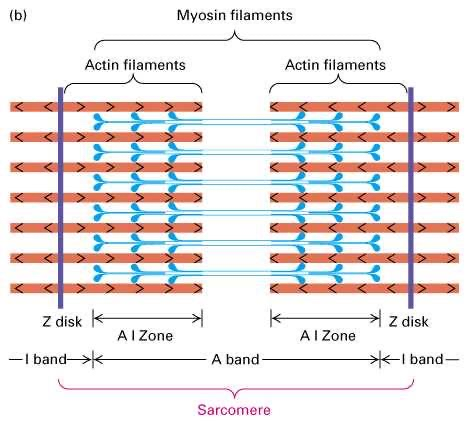
\includegraphics[width=0.5\linewidth]{sarcomere.jpeg}
    \caption{Sarcomere structure}
        \label{fig:placeholder}
\end{figure}

\subsubsection{H zone vs bare zone}

\begin{itemize}
    \item \textbf{H zone} : no actin
    \item \textbf{Bare zone} : region within the myosin filament where \textbf{myosin heads} are absent 
    \item The \textbf{{bare zone}} is essentially a structural feature of the \textbf{{myosin filament}}, whereas the \textbf{{H zone}} is a region of the \textbf{{sarcomere}}
\end{itemize}

\subsection{Thick and thin filaments}
\begin{itemize}
    \item \textbf{\textcolor{blue}{Myosin}} molecules aggregate from the center of the \textbf{\textcolor{blue}{thick filament}} by overlapping their tails and orienting their heads in opposite directions. In this way, a central region of the thick filament remains free of heads, the \textbf{bare zone}, and in the two half-filaments that extend from it the heads have an antiparallel orientation
    \item The \textbf{\textcolor{red}{thin filament}} is formed by the globular protein G-actin, which polymerizes into filamentous \textbf{\textcolor{red}{F-actin}}, and by the regulatory proteins \textbf{troponin (Tn)} and \textbf{tropomyosin (Tm)}.  It is anchored on the \textbf{Z discs}
    \item \textbf{Tropomyosin} lies in the groove between the two chains of the \textbf{\textcolor{red}{actin}} filament. It is a filamentous protein that covers the length of 7 actin monomers and polymerizes to form a filament extending along the entire actin filament. \textbf{Troponin}, a protein complex composed of three
    subunits, TnC, TnI and TnT, is located at the overlap between two
    adjacent \textbf{tropomyosin} monomers
    \item \textbf{Tropomyosin} physically blocks the binding sites on the \textbf{\textcolor{red}{actin}} filament
\end{itemize}

\subsection{Actin-myosin interaction}
\subsubsection{Cross bridges}
\begin{itemize}
    \item When the muscle is relaxed, the concentration of $\text{Ca}^{2+}$ in the cytoplasm is very \textbf{low}. On the \textbf{\textcolor{red}{actin}} filament, tropomyosin covers the binding sites for \textbf{\textcolor{blue}{myosin}}. Therefore, even though \textbf{\textcolor{blue}{myosin heads}} are ready to interact with \textbf{\textcolor{red}{actin}}, they cannot bind strongly to \textbf{\textcolor{red}{actin}}.
    \item A motor neuron releases \textbf{acetylcholine}, which causes an \textbf{action potential} in the muscle fiber. This triggers the sarcoplasmic reticulum (SR) to release $\text{Ca}^{2+}$ into the cytoplasm.
    \item The $\text{Ca}^{2+}$ binds specifically to \textbf{TnC}. This causes a conformational change in the \textbf{troponin–tropomyosin complex} (TnC undergoes a conformational change). As a result, it changes its interaction with the other troponin components, particularly TnI. As \textbf{tropomyosin} is linked to the \textbf{troponin complex} by TnT, it moves away from the myosin-binding sites on actin.
    \item Once the binding site is exposed, a \textbf{\textcolor{blue}{myosin head}} can bind to \textbf{\textcolor{red}{actin}}. This is the formation of a \textbf{cross-bridge}.
    \item ATP is hydrolyzed : $ \text{ATP} \rightarrow \text{ADP + } \mathrm{P_i}$ and the \textbf{\textcolor{blue}{myosin head}} is then in a high-energy, \textbf{cocked conformation}
    \item $\mathrm{P_i}$ is released, followed by ADP. The \textbf{\textcolor{blue}{myosin head}} changes its conformation and pulls the \textbf{\textcolor{red}{actin filament}} toward the \textbf{M line}. This is where mechanical force is generated.
    \item \textbf{Power stroke} : the \textbf{\textcolor{blue}{myosin head}} is essentially acting as a \textbf{molecular lever} 
    \item A new ATP binds to \textbf{\textcolor{blue}{myosin}}. This causes \textbf{\textcolor{blue}{myosin}} to release \textbf{\textcolor{red}{actin}}.
    \item ATP is hydrolyzed again and the energy released is used to return the \textbf{\textcolor{blue}{myosin head}} to its \textbf{cocked} position : a \textbf{new cycle} is then possible
    \item \textbf{Cross-bridges} are independent force generators that act in parallel in the half-sarcomere.
    \item if ATP is \textbf{absent} (rigor): There is no new ATP available to cause detachment. Therefore, the myosin head remains permanently locked onto the actin filament, frozen in its low-energy position at the exact end of the working stroke
    \item To sum up, the \textbf{Lymn-Taylor cycle} is composed of four stages and is during around 100  ms 
    \begin{enumerate}[label=(\arabic*)]
        \item \textbf{Attachment} — Myosin head (with ADP + Pi) binds to exposed actin.
        \item \textbf{Power stroke} — Pi and ADP are released → myosin changes shape and pulls actin toward the M line. It's a fast step, around 1 ms.
        \item \textbf{Detachment} — ATP binds to myosin → myosin releases actin.
        \item \textbf{Re-cocking} — ATP is hydrolyzed to ADP + Pi → myosin head returns to its high-energy position, ready to bind again.
    \end{enumerate}
    
\end{itemize}

\subsubsection{Myosin heads}

The myosin molecule can be divided into a \textbf{head region (S1 domain)} and a tail region. The tail consists of the \textbf{S2 domain}, which connects the heads to the \textbf{thick filament}, and the \textbf{Light Meromyosin (LMM) region}, which is incorporated \textbf{into the thick filament}.

\subsubsection{Thin filament activation}
\begin{itemize}
    \item Triggered by the presence or the absence of $\text{Ca}^{2+}$ in the cytosol which activate the \textbf{\textcolor{red}{actin}} sites to let the myosin heads bind
\end{itemize}

\subsubsection{Activation and relaxation}
\begin{itemize}
    \item \textbf{NCX} : Sodium / Calcium ions exchangers, primarily a membrane $\text{Ca}^{2+}$ extrusion pathway in cardiac muscle. Taking 3 $\text{Na}^{+}$ions from outside the cell to evacuate one $\text{Ca}^{2+}$ from the inside 
    \item  \textbf{SR} : the major intracellular $\text{Ca}^{2+}$ reservoir
    \item \textbf{RyRs} :  inwards calcium fluxes receptors and also release channels for calcium ions
    \item \textbf{SERCA} : a protein pump in the membrane of the SR, it is pumping $\text{Ca}^{2+}$ from the cytosol into the SR
    \item RyR $\rightarrow$ releases $\text{Ca}^{2+}$ from SR $\rightarrow$ contraction
    \item SERCA $\rightarrow$ puts $\text{Ca}^{2+}$ back into the SR $\rightarrow$ relaxation
    \item NCX $\rightarrow$ moves $\text{Ca}^{2+}$ out of the cell $\rightarrow$ helps relaxation
    \item  $\text{Ca}^{2+}$ leaves troponin C $\rightarrow$ tropomyosin blocks the actin binding sites again $\rightarrow$ cross-bridge cycling decreases $\rightarrow$ sarcomere relaxes.
    \item (1) he action potential travels on the membrane, (2) calcium ion channels are activated and let calcium ions in, (3) this calcium flux triggers the sarcoplasmic reticulum, (4) calcium is released in the cytosol, (5) calcium ions are captured by the sarcomere, (6) calcium ions are taken from the sarcomere, (7) calcium ions are uptaken by the sarcoplasmic reticulum or removed from the cells by the exchangers
\end{itemize}

\subsubsection{Titin}
\begin{itemize}
    \item A giant protein located into the sarcomere that connects the \textbf{Z-disc} to the \textbf{thick filament}, anchored in the \textbf{M-line}.
    \item Titin allows the sarcomere to recover its original length in the relaxation phase : when the sarcomere is stretched, titin extends and when the muscle is released, titin tends to return toward its original configuration.
    \item Titin acts as an elastic spring that generates passive tension, limits excessive sarcomere extension, and participates in mechanosensing
\end{itemize}


\subsection{The 3-Component Mechanical Model}
Hill's model simplifies muscle structure into three distinct parts, separating active engines from passive elastic springs:
\begin{itemize}
    \item \textbf{CC (Contractile Component):} The active \textbf{sarcomeres} (\textbf{\textcolor{red}{actin}} and \textbf{\textcolor{blue}{myosin}}) that actively generate force.
    \item \textbf{SEC (Series Elastic Component):} Passive springs in a \textbf{straight line} with the CC (\textbf{tendons}, titin, myosin heads). 
    \item \textbf{PEC (Parallel Elastic Component):} Passive springs \textbf{surrounding} the CC (\textbf{connective tissues}: epimysium, perimysium, endomysium). It protects the muscle during passive stretch.
\end{itemize}

\subsection{Isotonic Quick-Release Mechanics}
When a fully stimulated muscle is suddenly released against a lower, constant load (\textit{Isotonic Quick-Release}), the mechanical response occurs in two distinct, sequential phases:

\textbf{Phase 1: Instantaneous Response ($\rightarrow$ SEC)}

\begin{itemize}
    \item \textbf{Mechanism:} The sudden drop in load causes the muscle to snap back instantly. The active engine (CC) is too slow to react; this is purely passive spring recoil (\textbf{Force-Extension relationship})
    \item \textbf{Isolated Component:} The \textbf{SEC} (in-line springs) relaxing.
\end{itemize}

\textbf{Phase 2: Steady-State Response ($\rightarrow$ CC)}

\begin{itemize}
    \item \textbf{Mechanism:} Once the springs stabilize, the muscle continues to shorten at a constant, steady speed to move the remaining load.
    \item \textbf{Isolated Component:} The \textbf{CC} (active cross-bridge cycling).
    \item \textbf{Governing Law:} This phase maps the \textbf{Force-Velocity relationship} (Hill's Law: Heavy load = slow speed; Light load = fast speed).
\end{itemize}

\subsubsection{Isometric vs. Isotonic Contraction}
Muscle contractions are categorized based on changes in length and tension. The mechanical behaviors differ fundamentally between isometric and isotonic states:

\begin{itemize}
    \item \textbf{Isometric Contraction (Static):} The muscle develops tension but \textbf{does not change length}. The active contractile component (CC) shortens slightly just to stretch the series elastic component (SEC), but no external work is performed ($W = 0$).
    \item \textbf{Isotonic Contraction (Dynamic):} The muscle \textbf{changes length while maintaining constant tension} once the external load is overcome. This contraction performs external work and is governed by the force-velocity relationship.
    \item \textbf{Length Clamp} : The experimental system holds the overall length of the muscle (or a specific segment of sarcomeres) constant, or changes it in a precisely controlled step, allowing researchers to measure the resulting changes in tension
    \item \textbf{Load Clamp (Force Clamp)}: The system abruptly alters or maintains a constant external load on the muscle during contraction or relaxation, allowing researchers to observe how fast and how far the muscle shortens or lengthens under that specific load

\end{itemize}


\subsubsection{The Force-Velocity Relationship and Power Curves}
The force-velocity curve defines the physical limits of the active \textbf{Contractile Component (CC)}. To compare different muscle types, force ($T$) and velocity ($V$) are normalized against their maximum values ($T_0$ and $V_0$). Muscle power is the rate of doing work, expressed as the product of force and velocity

\begin{itemize}
    \item \textbf{Inverse Relationship:} Force and velocity share an inverse, hyperbolic relationship. As load ($T/T_0$) increases, shortening velocity ($V/V_0$) drops.
    \item \textbf{Peak Power Sweet Spot:} Maximum power output does not occur at maximum speed or force. \textbf{Maximum power peaks at approximately $1/3$ of maximum velocity ($V_0$) and force ($T_0$)}.
    \item \textbf{Fast Fibers vs. Slow Fibers:} Fast fibers maintain higher shortening velocities under load. They deliver a significantly \textbf{higher peak power output} than slow fibers.
    \item \textbf{Curve Customization:} The curvature of these relationships varies by muscle type, mathematically defined by Hill's normalized constants ($a/T_0$ and $b/V_0$).
\end{itemize}

\subsubsection{Heat Production During Contraction and the Fenn Effect}
Muscle contraction is \textbf{thermodynamically active} :

\begin{itemize}
    \item \textbf{Components of Heat (Graph a):} Heat production ($Q$) rises dramatically from rest ($1.6 \times 10^{-4}$ J g$^{-1}$ s$^{-1}$) to tetanic contraction ($10^{-2}$ J g$^{-1}$ s$^{-1}$). It is divided into:
    \begin{itemize}
        \item \textbf{Activation Heat:} The initial burst triggered at the onset of stimulus ($t_1$)
        \item \textbf{Maintenance Heat:} The steady, continuous heat produced during isometric contraction
        \item \textbf{Shortening Heat:} The additional heat generated when the muscle shortens isotonically ($t_2$)
    \end{itemize}
    \item \textbf{The Fenn Effect:} A muscle releases more total energy when allowed to shorten (isotonic) than when holding a fixed length (isometric). Shortening mobilizes extra metabolic energy.
    \item \textbf{Rate of Energy Release (Graph b):} The total rate of energy release increases monotonically with shortening velocity ($V/V_0$). It represents the mathematical sum of the active mechanical power ($W$) and the rate of heat release ($Q$).
\end{itemize}

\section{Poisson Random Measure}

A Poisson random measure (PRM) can be interpreted as a random collection
of points. For a measurable set $A$, define

\[
\boxed{
N(A)
=
\text{number of Poisson points contained in }A
}
\]

or, more formally, if the random points are $(X_i)_{i\geq1}$,

\[
\boxed{
N(A)
=
\sum_{i\geq1}\mathbf{1}_{\{X_i\in A\}}.
}
\]

The random measure $N$ is a Poisson random measure with intensity measure
$\nu$ if

\[
\boxed{
N(A)\sim\operatorname{Poisson}\bigl(\nu(A)\bigr)
}
\]

for every measurable set $A$.

Hence,

\[
\mathbb{E}[N(A)] = \nu(A),
\qquad
\operatorname{Var}(N(A)) = \nu(A).
\]

Moreover, if $A_1,\ldots,A_n$ are disjoint,

\[
A_i\cap A_j=\varnothing
\qquad (i\neq j),
\]

then

\[
\boxed{
N(A_1),\ldots,N(A_n)
\text{ are independent}.
}
\]

\subsection{Connection with the Poisson process}

If the PRM is defined on the time axis $\mathbb{R}_+$ with

\[
\boxed{
\nu(dt)=\lambda\,dt,
}
\]

then

\[
N([s,t])
\sim
\operatorname{Poisson}\bigl(\lambda(t-s)\bigr).
\]

The associated Poisson process is simply

\[
\boxed{
N_t=N([0,t]).
}
\]

Thus, the Poisson process counts the number of points of the PRM
that have occurred before time $t$.

\subsection{Marked Poisson Random Measure}

If each event has a time $t$ and an additional mark $z$, we consider

\[
\boxed{
N(dt,dz).
}
\]

For a region $A\subset\mathbb{R}_+\times\mathbb{R}_+$,

\[
N(A)
=
\text{number of points }(t,z)\text{ contained in }A.
\]

For example, if

\[
A=[t,t+dt]\times[0,\lambda(t)],
\]

and the PRM has intensity

\[
\nu(dt,dz)=dt\,dz,
\]

then

\[
\mathbb{E}[N(A)]
=
\int_t^{t+dt}\int_0^{\lambda(r)} dz\,dr
\simeq
\lambda(t)\,dt.
\]

Therefore, keeping only the points satisfying

\[
\boxed{
z\leq\lambda(t)
}
\]

generates events with instantaneous rate $\lambda(t)$.
This procedure is called \textbf{Poisson thinning}.

\subsection{Application to attachment/detachment}

For a myosin head,

\[
\alpha_t\in\{0,1\},
\]

with

\[
\alpha_t=
\begin{cases}
0, & \text{detached},\\
1, & \text{attached}.
\end{cases}
\]

We introduce two independent PRMs,

\[
N_{0\to1}(dt,dz),
\qquad
N_{1\to0}(dt,dz),
\]

for attachment and detachment events.

The attachment rate is $f(s(t))$ and the detachment rate is $g(s(t))$.
Thus,

\[
d\alpha_t
=
(1-\alpha_{t-})
\int_{\mathbb{R}_+}
\mathbf{1}_{\{z\leq f(s(t))\}}
N_{0\to1}(dt,dz)
\]

\[
\hspace{2cm}
-
\alpha_{t-}
\int_{\mathbb{R}_+}
\mathbf{1}_{\{z\leq g(s(t))\}}
N_{1\to0}(dt,dz).
\]

The indicators ensure that

\[
0\xrightarrow{f(s(t))}1,
\qquad
1\xrightarrow{g(s(t))}0.
\]

Hence the PRM provides the random events, while the functions
$f(s(t))$ and $g(s(t))$ determine their rates.


\subsection{Simulation of Myosin Head Mechanics via Alternating Inhomogeneous Poisson Processes}

The state of a myosin head is modeled as a two-state stochastic process $\alpha_t \in \{0, 1\}$, where:
\begin{itemize}
    \item $\alpha_t = 0$ represents the \textbf{detached state}.
    \item $\alpha_t = 1$ represents the \textbf{attached state}.
\end{itemize}

The position variable $s(t)$ represents the location of the closest actin site relative to the myosin head, moving at a given sliding speed $\dot{s}(t) = \dot{x}_c(t)$. The stochastic transitions between these two states are governed by time-inhomogeneous rates that depend directly on $s(t)$:

\begin{enumerate}
    \item \textbf{Attachment ($0 \rightarrow 1$):} When detached ($\alpha_t = 0$), the probability of attaching in an infinitesimal window $[t, t + \delta t]$ is given by:
    \begin{equation}
        \mathbb{P}(\alpha_{t+\delta t} = 1 \mid \alpha_t = 0) = f(s(t))\delta t + o(\delta t)
    \end{equation}
    The waiting time $\Delta T_t$ until the next attachment satisfies:
    \begin{equation}
        \mathbb{P}(\Delta T_t \leq t') = 1 - \exp\left( -\int_{t}^{t+t'} f(s(r)) \, dr \right)
    \end{equation}

    \item \textbf{Detachment ($1 \rightarrow 0$):} When attached ($\alpha_t = 1$), the probability of detaching in $[t, t + \delta t]$ is given by:
    \begin{equation}
        \mathbb{P}(\alpha_{t+\delta t} = 0 \mid \alpha_t = 1) = g(s(t))\delta t + o(\delta t)
    \end{equation}
\end{enumerate}

\subsubsection{The Thinning Simulation Strategy}
Because the transitions alternate and rely on time-dependent intensity functions $f(s(t))$ and $g(s(t))$, we can simulate the trajectory using a state-dependent thinning approach:
\begin{enumerate}
    \item Find upper bounds for the rate functions over the simulation horizon: $f_{\max} \geq f(s(t))$ and $g_{\max} \geq g(s(t))$.
    \item If the current state is $\alpha_t = 0$, propose a candidate jump time $\Delta t \sim \text{Exp}(f_{\max})$. Accept the attachment event with probability $\frac{f(s(t + \Delta t))}{f_{\max}}$.
    \item If the current state is $\alpha_t = 1$, propose a candidate jump time $\Delta t \sim \text{Exp}(g_{\max})$. Accept the detachment event with probability $\frac{g(s(t + \Delta t))}{g_{\max}}$.
\end{enumerate}

\section{Curie Weiss and collective behavior}

\subsection{Soft device}

\begin{figure}
    \centering
    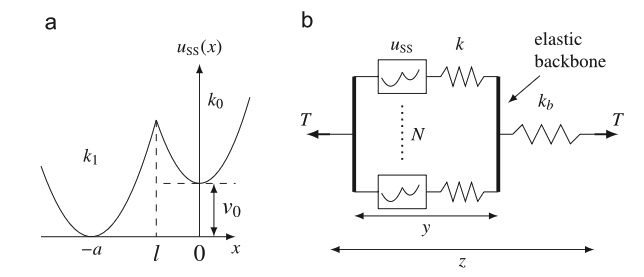
\includegraphics[width=0.7\linewidth]{snap_spring.png}
    \caption{Hard spin model of a parallel bundle of bistable crosslinkers}
        \label{fig:placeholder}
\end{figure}

\begin{itemize}
    \item $y$ : elongation of the cluster of parallel cross-bridges 
    \item $\sigma$ : tension per cross-bridge 
    \item $N\sigma$ : global force exerted by the entire system of $N$ cross-bridges 
    \item $x_i = \lbrace 0,1\rbrace$
    \item $\sigma$ couples only to the macroscopic state and does not multiply the individual elements $x_i$ directly so the $x_i$'s feel the tension \textbf{indirectly} 
\end{itemize}
\begin{equation}
    w (\lbrace x\rbrace, y \, ; \sigma) = \frac{1}{N} \sum_{i=1}^N \,\left\lbrace (1+x_i)v_0 + \frac{1}{2} (y-x_i)^2 - \sigma y \right\rbrace
\end{equation}
\begin{itemize}
    \item We are looking for a minimization of the energy with respect to $y$, going from $w (\lbrace x\rbrace, y \, ; \sigma)$ to $w (\lbrace x\rbrace ; \sigma)$
\end{itemize}

\begin{align*}
    \partial_y w = 0 &\Longleftrightarrow \partial_y \left( \frac{1}{N} \sum_{i=1}^N \,\left\lbrace (1+x_i)v_0 + \frac{1}{2} (y-x_i)^2 - \sigma y \right\rbrace \right) = 0 \\
    &\Longleftrightarrow \frac{1}{N} \sum_{i=1}^N \left( (y-x_i) - \sigma \right) = 0 \\
    &\Longleftrightarrow y - \frac{1}{N} \sum_{i=1}^N x_i - \sigma = 0 \\
    &\Longleftrightarrow y = \bar{x} + \sigma
\end{align*}
So that 
\begin{equation}
    \boxed{y^* = \sigma + \frac{1}{N}\sum_i x_i}
\end{equation}

Introducing the discrete order parameter $p = - \frac{1}{N} \sum_i x_i$, the fraction of the cross-bridges in the \textit{folded} state, the energy $\hat{w} (\lbrace x \rbrace ; \sigma)$ is

\begin{align*}
    \hat{w} (\lbrace x \rbrace ; \sigma) &= \frac{1}{N} \sum_{i=1}^N \,\left\lbrace (1+x_i)v_0 + \frac{1}{2} (\sigma + \frac{1}{N}\sum_i x_i -x_i)^2 - \sigma \left(\sigma + \frac{1}{N}\sum_i x_i \right) \right\rbrace \\
    &=  \frac{1}{N} \sum_{i=1}^N \,\left\lbrace (1+x_i)v_0 - \frac{\sigma^2}{2} -\sigma x_i -\frac{x_i}{N}\sum_i x_i + \frac{x_i}{2}^2 + \frac{1}{2}\left(\frac{1}{N}\sum_i x_i \right)^2  \right\rbrace \\
    & = (1-p) v_0 -\frac{1}{2}\sigma^2 + \sigma p + \frac{1}{N}\sum_i x_ip + \frac{1}{2N}\sum_i x_i^2 + \frac{p^2}{2} \\
    & = -\frac{1}{2}\sigma^2 + \sigma p -\frac{p^2}{2} + \frac{p}{2} + (1-p)v_0 \\
    & = -\frac{1}{2}\sigma^2 + \sigma p + \frac{p}{2}(1-p) + (1-p)v_0
\end{align*}
 using $\sum_i x_i^2 = \sum_i x_i$ because $x_i =\lbrace0,1\rbrace$. Thus there is a coupling term $p(1-p)$ traducing the mean-field interaction between the individual cross-bridges

We derive the metastable states from

\begin{equation}
    \hat{z} = -\partial_{\sigma} \hat{w} (p ; \sigma) =\sigma - p
\end{equation}
Furthermore, we are looking at the global extrema using 

\begin{equation}
    \partial^2_{\sigma} \hat{w} = - \partial_{\sigma} \hat{z} = - 1 < 0 
\end{equation}
which means that the energy $\hat{w}$ is concave in p and admits a global minimum for $p =0 $ or $p=1$. 
It also shows the sharp transition for $\sigma = \sigma^* = v_0$ where we can observe a \textit{bistable} state 

\begin{equation}
    \hat{w}(p ; \sigma^*) = -\frac{1}{2} v_0^2 + v_0 \text{ for p = 0 or 1}
\end{equation}

\begin{figure}
    \centering
    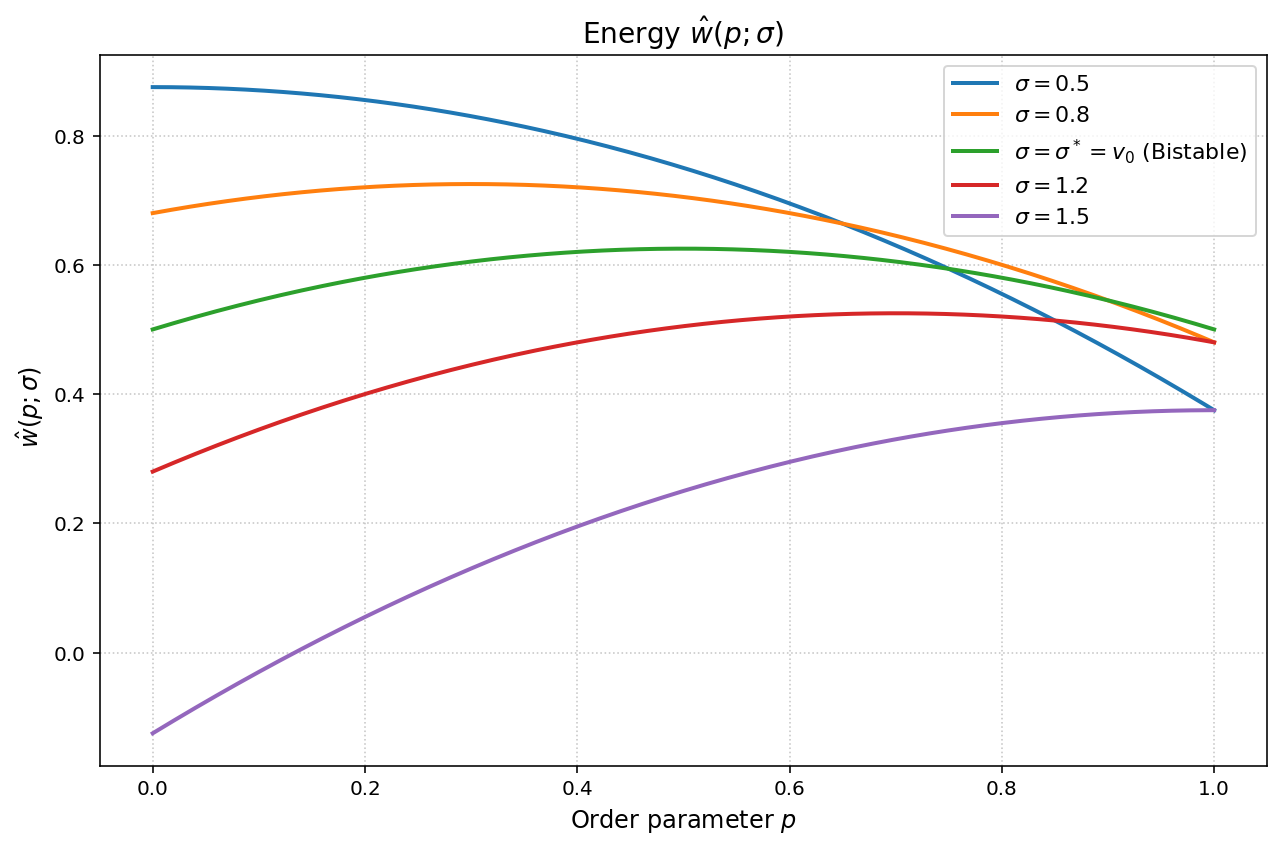
\includegraphics[width=0.45\linewidth]{energies_w_hat.png} 
    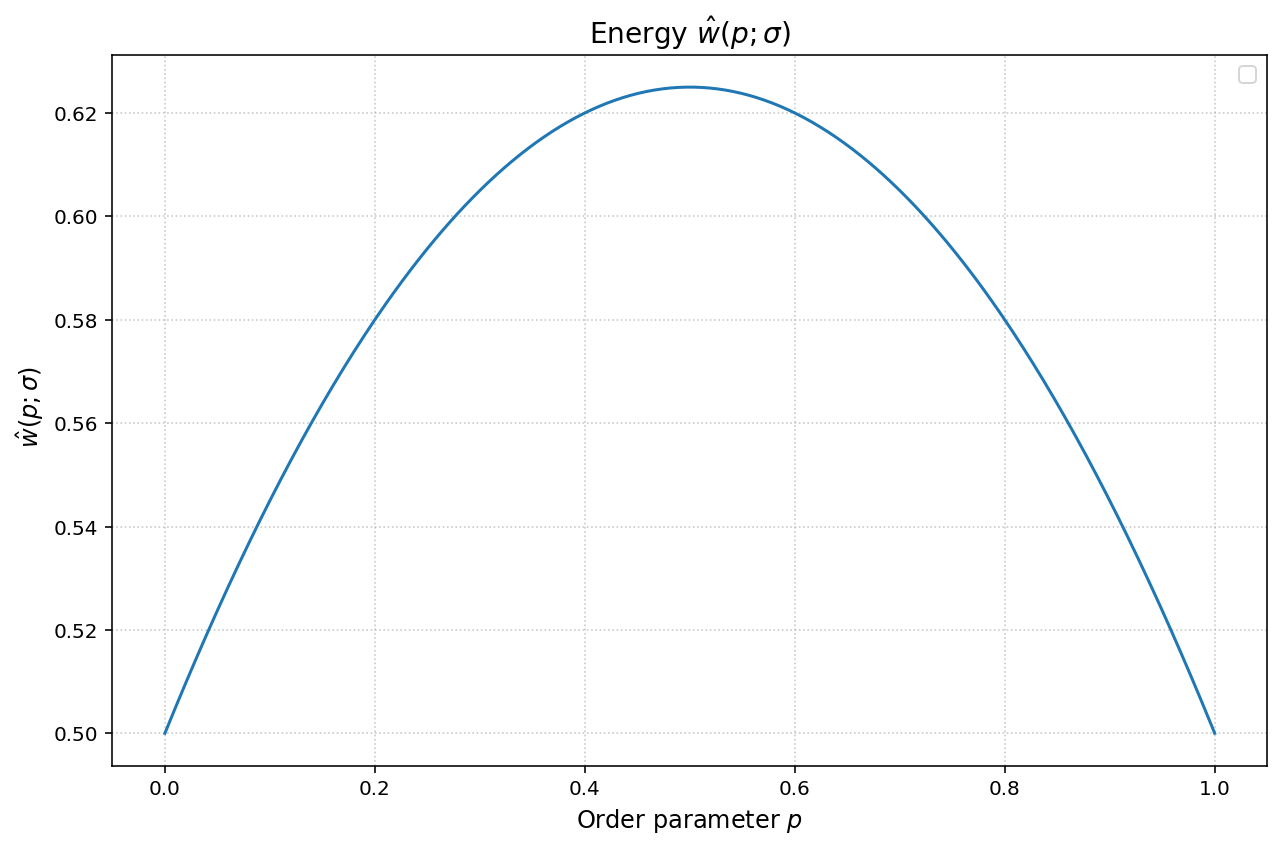
\includegraphics[width=0.45\linewidth]{energy_w_hat_one_value.png} 
    \caption{Energies $\hat{w}$ for several $p$ values}
    \label{fig:placeholder}
\end{figure}

\section{Soft Device framework}

We want to compare two different setups of the soft device framework, one with a number $N$ finite of myosin heads and one with an inifinite number of independent heads.

\subsection{h-model framework for N finite}

In the context of the soft device framework where the total tension $\Sigma_{ext}$ is prescribed, we consider a system of $N$ myosin heads. The position of each is represented by a random variable $X_t^i$ and the attachment state described by a discrete variable $\alpha_t^i \in \{0, 1\}$, where $0$ corresponds to the detached state with an energy $w_0$ and $1$ corresponds to the attached one with an energy $w_1$.\\
We consider a total number of $P$ actin sites separated by a distance $d$ per filament and the position of the closest actin site to the myosin head is denoted by $s_t^i = X_t^i + h_t^i $. The position over the actin filament is parameterized by the variable $y$.
We introduce the new variable representing the external force applied per head $N\sigma = \Sigma_{ext}$ and the total force exerted by the $N$ myosin motors is $F_{mot} = \sum_i f_i = \sum_{i=1}^N \alpha_t^i \partial_x(X_t^i)$. 
The force exerted by each myosin head derives from the energy of the spring $f_i = -\nabla E_i(X_t^i) = -k{X_t^i}^2$ where $k$ is the stiffness of the spring.\\ 
The dynamics of the system is then described by the following set of equations at equilibrium :
\begin{equation}
    \Sigma_{ext} + F_{mot} - \nu \dot{y}= 0
\end{equation}
where $\nu \dot{y}$ is the macroscopic viscous drag. The dynamics of the myosin heads can be written as

\begin{equation}
    N \sigma + N f - \nu \dot{y} = 0 \quad \text{with} \quad f = -\frac{k}{N} \sum_{i=1}^N \alpha_t^i X_t^i
\end{equation}
\subsubsection{ Dimensionless h-model framework with N finite}

We want to wrote the h-model framework in a dimensionless form. We use $kd$ as the force scale, $d$ as the length scale and $\tau$ as the time scale. We introduce the following dimensionless variables :
\begin{equation}
    \tilde{X}_t^i = \frac{X_t^i}{d}, \quad \frac{d\tilde{y}}{d\tilde{t}} = \frac{dy}{dt}\frac{\tau}{d}, \quad \tilde{\sigma} = \frac{\sigma}{kd}, \quad \tilde{f} = \frac{f}{kd}
\end{equation}
so that the dimensionless form of the dynamics of the system is
\begin{equation}
    \tilde{\sigma} + \tilde{f} - \frac{\nu}{Nk\tau} \frac{d\tilde{y}}{d\tilde{t}} = 0
\end{equation}

We now write the dynamics for one motor in the detached state in dimensionless form, using $kd^2$ as the energy scale and $\tau$ as the time scale.
\begin{equation}
    dX_t^i = - \frac{1}{\eta}\left. \frac{dw_0}{dx} \right|_{x = X_t^i} dt + \sqrt{\frac{2k_B T}{\eta}} dB_t^i
\end{equation}
Introducing the dimensionless variables 
\begin{equation}
    d\tilde{X}_t^i = \frac{dX_t^i}{d} \quad \tilde{t} = \frac{t}{\tau} \quad \frac{\tilde{w}_0}{\tilde{x}} = \frac{dw_0}{dx}\frac{d}{kd^2} \quad \tilde{B}_t^i = \frac{B_t^i}{\sqrt{\tau}}
\end{equation}
The dimensionless form of the dynamics for one motor in the detached state is then
\begin{equation}
    d\tilde{X}_t^i = - \frac{k\tau}{\eta}\left. \frac{d\tilde{w}_0}{d\tilde{x}} \right|_{\tilde{x} = \tilde{X}_t^i} d\tilde{t} + \sqrt{\frac{2\beta k\tau}{\eta}} d\tilde{B}_t^i \qquad \beta = \frac{k_B T}{k d^2}
\end{equation}
We then have two possibilities for the characteristic time $\tau$ : either we choose $\tau = \frac{\eta}{k}$ or $\tau = \frac{\nu}{k}$. In the first case, we have a microscopic timescale while in the second case this is a macroscopic timescale.\\
We choose the first case, so that all dependencies are captured in the dimensionless form of the macroscopic equation and keeps the detached-head dynamics independent of the viscosity ratio $\gamma$ as 
\begin{equation}
    d\tilde{X}_t^i = - \left. \frac{d\tilde{w}_0}{d\tilde{x}} \right|_{\tilde{x} = \tilde{X}_t^i} d\tilde{t} + \sqrt{2\beta} d\tilde{B}_t^i
\end{equation}
\begin{equation}
    \tilde{\sigma} + \tilde{f} - \frac{\gamma}{N} \frac{d\tilde{y}}{d\tilde{t}} = 0 \quad \text{with} \quad \gamma = \frac{\nu}{\eta}
\end{equation}
The limits can thus be interpreted as follows 
\begin{itemize}
    \item $\gamma \rightarrow 0$ : the macroscopic drag is negligible compared to the microscopic viscosity, so that the system is dominated by the microscopic dynamics of the myosin heads and the force balance becomes a singular constraint $\tilde{\sigma} + \tilde{f} = 0$ for a finite limiting velocity.
    \item $\gamma \rightarrow \infty$ : the macroscopic drag is dominant compared to the microscopic drag, so that the system is dominated by the macroscopic dynamics of the myosin heads. For bounded forces; the filament velocity is negligible and the system is quasi-static.
\end{itemize}

For the dynamics of the attached state, we have
\begin{equation}
    dX_t^i = \dot{y} dt
\end{equation}
so that the dimensionless form of the dynamics for one motor in the attached state is
\begin{equation}
    d\tilde{X}_t^i = \frac{d\tilde{y}}{d\tau} d\tau
\end{equation}
The periodic coordinate satisfies $dh_t^i = \dot{y} dt - d\pi(X_t^i)$ and the dimensionless form is
\begin{equation}
    d\tilde{h}_t^i = \frac{d\tilde{y}}{d\tau} d\tau - d\tilde{\pi}(\tilde{X}_t^i)
\end{equation}


\subsubsection{jumps in the h-model framework with N finite}
The jumps in the h-model framework with N finite are modeled using two independent Poisson random measures for the two transitions $N_+^i(dt,dh,du)$ and $N_-^i(dt,dh,du)$, with intensity $\nu(dt\,dh\,du) = dtdhdu$.\\
Let's The dynamics of the attachment/detachment process is then given by
\begin{equation}
\begin{aligned}
d\alpha_t^i &= d\alpha_t^i\Big|_+ + d\alpha_t^i\Big|_- \\
&= \mathbf{1}_{\{\alpha_{t^-}=0\}} \int_{\mathbb{R}_+ \times \mathbb{T}_d} \mathbf{1}_{\{u \le k_{0+}(X_{t^-}^i, h)\}} N_+^i(dt, dh, du) \\
&\quad - \mathbf{1}_{\{\alpha_{t^-}=1\}} \int_{\mathbb{R}_+ \times \mathbb{T}_d} \mathbf{1}_{\{u \le k_{0-}(X_{t^-}^i, h)\}} N_-^i(dt, dh, du)
\end{aligned}
\end{equation}

We choose a truncated normalized Gaussian density for the rate $k_{0+}(X_{t^-}^i, h)$, as the attachment is preferentially localized around the actin site on the filament, and an uniform detachment rate $k_{0-}(X_{t^-}^i, h)$ over the whole window considered.  
The rates can then be written as
\begin{equation}
    k_{0+}(x, h) 
=\lambda_+(x)\,q_G(h)
\quad \text{where} \quad q_G(h)=
\frac{\exp(-h^2/(2\sigma^2))}
{\displaystyle\int_{-d/2}^{d/2}\exp(-u^2/(2\sigma^2))\,du}
\mathbf 1_{\{|h|\le d/2\}}
\end{equation}
$\lambda_+(x)$ is the total attachment rate for a myosin head at position $x$ and $q_G(h)$ is the truncated Gaussian distribution centered on the actin site. 
The detachment rate is uniform over the window considered, so that we can define 
\begin{equation}
    k_{0-}(x, h) = \lambda_-(x)\,q_U(h) = \frac{\lambda_-(x)}{d}\mathbf 1_{\{|h|\le d/2\}} \quad \text{where} \quad q_U(h) = \frac{1}{d}\mathbf 1_{\{|h|\le d/2\}}
\end{equation}
Using $d$ as the characteristic length scale and $\tau$ as the characteristic time scale, we can write the dynamics of the attachment/detachment process in dimensionless form as
\begin{equation}
\tilde k_{0+}=t_0d\,k_{0+},
\qquad
\tilde k_{0-}=t_0d\,k_{0-}.
\end{equation}
so that the window becomes $\tilde{h} \in [-1/2, 1/2]$ and the truncated Gaussian distribution is
\begin{equation}
\tilde{q}_G(\tilde{h})=
\frac{\exp[-\tilde h^2/(2\tilde\sigma^2)]}
{\displaystyle\int_{-1/2}^{1/2}
\exp[-r^2/(2\tilde\sigma^2)]\,dr},
\qquad
\tilde\sigma=\frac{\sigma}{d}
\end{equation}
while normalized dimensionless uniform density is simply
\begin{equation}
\tilde q_U(\tilde h)=\mathbf 1_{[-1/2,1/2]}(\tilde h).
\end{equation}

\subsection{h-model framework for N infinite}

We consider a system of $N$ independent myosin heads in the limit $N \to \infty$. For one single head, the force is 
\begin{equation}
    f_t=-\mathbf 1_{\alpha_t=1}\partial_xw_1(X_t).
\end{equation}
Let $p(t, 1, x)$ be the joint probability density of the head being attached and having coordinate $x$ at time $t$
\begin{equation}
    p(t,1,x)\,dx
=\mathbb P(\alpha_t=1,\ X_t\in[x,x+dx])
\end{equation}
Taking the expected value of the force over the distribution of the head's state and position, we have
\begin{equation}
    \mathbb E[f_t]
=-\int_{\mathbb R}\partial_xw_1(x)p(t,1,x)\,dx = -\tau_c(t)
\end{equation}
Therefore, assuming the heads are independent and identically distributed, the law of large numbers implies that the average force per head converges to the expected value as $N \to \infty$:
\begin{equation}
\frac1N\sum_{i=1}^N f_t^i
\longrightarrow -\int_{\mathbb R}\partial_xw_1(x)p(t,1,x)\,dx =-\tau_c(t)
\end{equation}
Writing the soft device macroscopic equation, we have 
\begin{equation}
    \Sigma_{ext} + \sum_i f_t^i - \nu \dot{y}= 0 
\end{equation}
In the infinite-population limit, $N \to \infty$, the limiting force balance per head is thus 
\begin{equation}
    \sigma - \tau_c(t) - \frac{\nu}{N}\dot{y} = 0
\end{equation}



\end{document}  